\begin{minipage}[t]{170mm}
\vspace{3mm}
\section{Ikke-kommutativ studenterrådgivning}
\emph{Kære brevkasse}

\emph{Min ven fortæller mig, at medmindre man har set på noget i mere end $4$ sekunder, så må man ikke udtale sig om hvordan det ser ud.}

\emph{Jeg forstår det ikke. Hvorfor?}

\emph{Hilsen den forundrede, der ser noget i 2,25 sekunder}

\subsection*{Svar}

\vspace{1mm}
\section*{IMO 2012 opgave 3}
Løgnerens gætteleg er et spil for to spillere A og B. Spillets regler bygger på to positive
heltal $k$ og $n$ som begge spillere kender. Ved spillets start vælger A hele tal $x$ og $N$, så $1 \le x \le N$. Spiller A holder $x$ hemmelig, men fortæller sandfærdigt spiller B hvad $N$ er. Derefter prøver spiller B at få information om $x$ ved at stille spiller A spørgsmål på følgende måde: Hvert spørgsmål består af at B vælger en vilkårlig mængde $S$ af positive heltal (evt. en som han allerede har valgt før) og spørger A om $x$ tilhører $S$. Spiller B må stille så mange spørgsmål han vil. Efter hvert spørgsmål skal spiller A omgående svare ja eller nej, men hun må lyve så mange gange hun har lyst til. Den eneste begrænsning er at der blandt vilkårlige $k + 1$ på hinanden følgende svar skal være mindst et svar som er sandt. Efter at B har stillet så mange spørgsmål som han vil, skal han angive en mængde $X$ med højst $n$ positive heltal. Hvis $x$ tilhører $X$, vinder B; og hvis ikke, taber han. Vis at:
\begin{enumerate}
\item[0.] Vis at hvis $k=1$ og $n=2$, har B en vindende strategi.
\item[1.] Hvis $n \ge 2^k$ , da har B en vindende strategi.
\item[2.] For alle tilpas store $k$ findes der et heltal $n \ge 1,99^k$, så B ikke har en vindende strategi.
\end{enumerate}

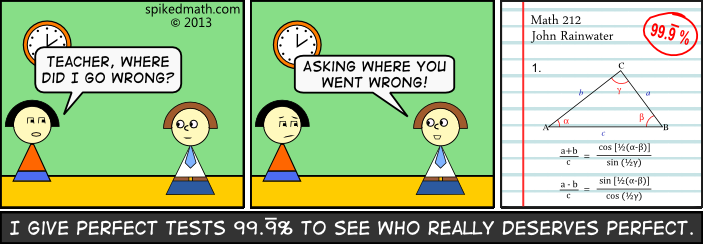
\includegraphics[width=\linewidth]{547-the-perfect-score.png}
\begin{center}
\tiny Mike, http://http://spikedmath.com/547.html, CC-BY-NC-2.5
\end{center}
\end{minipage}
